\documentclass{beamer}
% \usepackage{mathtools}
% \usepackage{color}
% \usepackage{pgfpages}
% \pgfpagesuselayout{4 on 1}[a4paper, border shrink=5mm, landscape]
% \usepackage{listings}
% \usepackage{minted}
% \usetheme{Madrid}
% \usetheme{Boadilla}
% \usetheme{Warsaw}
% \usetheme{Bergen}
% \usetheme{Amsterdam}
\usetheme{default}
\usecolortheme{beaver}
% \usepackage[number]{natbib}
\usepackage{natbib}


\title[CP]{L5DC Computing Project}
\subtitle{Project proposal}
\author{Achyut Timsina}

\date{\today}
\institute[Softwarica]{Softwarica college of IT \& E-Commerce\\
Kathmandu, Nepal\\
\url{actimsina@gmail.com}
}
\begin{document}

\maketitle

\section{Computing project introduction} % (fold)
\label{sec:computing_project_introduction}

\begin{frame}[t]\frametitle{Computing project's importance}
\begin{itemize}
    \item Culmination of two years of education
    \item Combines all of your knowledge till date to produce something useful 
\end{itemize}
\end{frame}

\begin{frame}[t]\frametitle{Tasks overview}
The project is divided into a number of sub-task as follows:
\begin{enumerate}
    \item Project proposal
    \item Analysis specification
    \item Design specification
    \item Midway presentations
    \item Final report
    \item Final presentation 
    \item Demonstration
\end{enumerate}
\end{frame}

\begin{frame}[t]\frametitle{Assignment rules}
\begin{itemize}
    \item All reports (doc/pdf) should be named as batch\_firstName\_lastName\_taskName\_version, For example: 9\_ram\_shrestha\_proposal.pdf(doc)
    \item Plagiarism will not be tolerated, and you have to submit your report to \url{www.turnitin.com} for the plagiarism check!
    \item Use Harvard style for referencing.
    \item All assignments hard copy and soft copy should be submitted with in respective deadlines.
    \item The deadlines are strict!
    \item The deadlines are published at computing project's site.
    \item Failure to submit assignments on the published deadlines will result in failing the course!
    \item Goal is to make you working continuously towards completion of projects on time with vibrant results!
    \item Email address for all of your digital communications is \textbf{cpsoftwarica@gmail.com}. I will try to write back with in 24 hours.
\end{itemize}
\end{frame}
% section computing_project_introduction (end)

\section{Project Scoping} % (fold)
\label{sec:scoping}

\begin{frame}[t]\frametitle{Project selection}
\begin{itemize}
    \item Most difficult stages of all
    \item Ideally have a real client for the software project
    \item (If you do not have real client, ) Try to be as practical as possible! (Try to solve practical problems)
    \item Your motivation level differs whether you have real client/project or not!
    \item You can look up the potential list of topics for projects.
    \item No two students can have exactly the same computing project topic.
\end{itemize}
\end{frame}

\begin{frame}[t]\frametitle{Project Scoping}
Project scoping report should consist of:
\begin{description}
    \item[Background]: What your project is about? Describe the area/domain of the project. Provide background and description of related concepts in your project. This section should set the scene for the project. \\

    What problem you are trying to solve? Why solving those problems matter? How you are going to solve identified problem(s)?

    \item[Main features]:
    What are the main functionalities that your project going to have? What will be your choice of programming language(s), tools, libraries for developing this project?
\end{description}
\end{frame}

\begin{frame}[t]\frametitle{Scoping (contd.)}
    \begin{description}
        \item[Aims and Objectives]:
    State a few major goals/aims of your project. For example:
    \emph{To build desktop application for managing student information system of ABC college}
    \emph{To make the student information more accessible at ABC college}\\

    Your objectives should be SMART:
    \begin{itemize}
        \item Specific
        \item Measurable
        \item Appropriate
        \item Realistic
        \item Time-related
    \end{itemize}
    \end{description}
\end{frame}

\begin{frame}[t]\frametitle{Scoping (contd.)}
    State objectives that corresponds to the stated aim(s).  Some of your objective can be academic, technical as well. For example:
    \begin{itemize}
        \item To analyze the student information management system
        \item To design the ...
        \item To develop ...
        \item To test ...
        \item To document ...
        \item To report ...
        \item To apply test driven development (TDD) ...
    \end{itemize}
Note: Refer to `sample\_proposal.pdf' at the FTP server!
\end{frame}

\section{Project Planning} % (fold)
\label{sec:project_planning}
\begin{frame}[t]\frametitle{Project Planning}
Project planning includes:
\begin{description}
        \item [Work breakdown structure (WBS)] produce a model that shows the tasks that must be completed in order to complete the project
        \item [Time estimates] produce estimates of the time required to complete the tasks
        \item [Milestones] Significant point in your project that can be used to give an indication of how well the project is going
        \item [Activities] Identify the order in which tasks must be completed
        \item [Present your plan] Use the tasks, time estimates, milestones and activities to produce a plan, normally in the form of a Gantt chart
        \item [Re-plan] if required adapt your plan to changing situation
    \end{description}
\end{frame}


\begin{frame}[t]\frametitle{Work breakdown structure (WBS)}
\begin{itemize}
        \item WBSs are used to break project down into lower and lower levels of details to reveal exactly what work will be done to complete the project.
        \item Begin WBS by breaking your projects down into its main  objectives (from aims/objectives)
        \item Continue breaking down the objectives down into lower and lower level of detail
        \item General guideline is to break the activities such a that the effort required to finish the activity is not less than 5\% of the total project effort.
        \item For a six month project, a WBS activity should not be less than one week of the time
        \item The total project management activity should not be greater than 10\% of the total project's effort.
        \item for a six month project, the total project management effort should not be greater than 2 weeks
    \end{itemize}
\end{frame}

\begin{frame}[t]\frametitle{Time estimates}
    \begin{itemize}
        \item Produce estimates of the time required to complete the tasks
        \item Fix deadline (April 15, 2015!)
        \item By breaking down into smaller activities, the time estimation will be more accurate (explain with example)
        \item Be flexible to adapt your time estimates based on the fixed delivery date.
        \item add up if conservative, reduce if lax (but your deadline is fixed)!!
    \end{itemize}
\end{frame}

\begin{frame}[t]\frametitle{WBS and Time estimates}
\begin{table}[htb!]
    \caption{Work breakdown structure with time estimate}
    \label{tab:wbs}
    \begin{center}
        \begin{tabular}{p{2cm}|l|l}
        \textbf{WBS \#} & \textbf{Task name} & \textbf{Days} \\
        \hline

        \hline
        1. & Your project name & 66\\
        \hline

        \hline
        1.1 & Project Management & 15 \\
        1.1.1 & Scoping & 5\\
        1.1.2 & Planning & 5\\
        1.1.3 & Monitoring \& Controlling & 5\\
        \hline
        1.2 & Analysis & 15 \\
        1.2.1 & Requirements & 5 \\
        1.2.2 & Use cases & 5 \\
        1.2.3 & Architecture & 5 \\
        \hline
        1.3 & Design & 15\\
        \hline
        1.4 & Testing & \\
        \hline
        1.5 & Reporting & \\
        \hline

        \hline
        \end{tabular}
    \end{center}
\end{table}
\end{frame}



% \begin{frame}[t]\frametitle{WBS example}
% \begin{figure}
%     \centering
%     \includegraphics[width = 0.9\textwidth]{sample_wbs}
%     \caption{An example WBS for a artificial neural network project}
%   \end{figure}
% \end{frame}
% frame time estimates


% \begin{frame}[t]\frametitle{Time estimates example}
%  \begin{figure}
%     \centering
%     \includegraphics[width = 0.9\textwidth]{time_estimates}
%     \caption{An example Time estimates for a artificial neural network (ANN) project}
%   \end{figure}
% \end{frame}

% frame milestones
\begin{frame}[t]\frametitle{Identify milestones}
    \begin{itemize}
        \item Milestones are significant steps towards the completion of a project.
        \item Help us to measure progress by providing intermediate reference points.
        \item Milestones can be identified by looking into the WBS!
        \item Milestones have a fix delivery date!
        \item Milestones are not activities, they are result or output of a activity.
        \item Refer to the milestones sections in the sample\_proposal report
    \end{itemize}
\end{frame}

% frame Activity sequencing
\begin{frame}[t]\frametitle{Activity sequencing}
\begin{itemize}
        \item Activity sequencing identifies the order in which the tasks should be performed.
        \item Also referred to as PERT networks, or network diagrams.
        \item Activity-on-nodes vs Activity on-arrow networks
        \item But we will use activity-on-nodes network diagram
    \end{itemize}
\end{frame}

% Scheduling
\begin{frame}[t]\frametitle{Scheduling}
\begin{itemize}
        \item Gantt charts!
        \item Show the durations of activities and identify instances when tasks are performed simultaneously
        \item Project activities are represented by rectangles or nodes
        \item The length of the rectangle shows the duration of the activity
        \item Milestones are represented by diamonds
    \end{itemize}
\end{frame}

\begin{frame}[t]\frametitle{Gantt Chart}
\begin{figure}[htb!]
    \begin{center}
        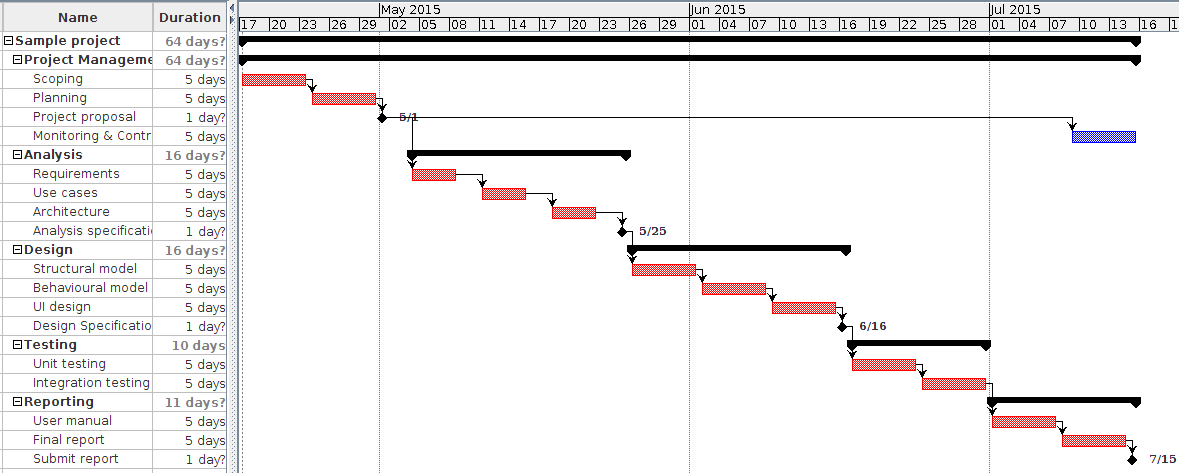
\includegraphics[width=6in]{../img/sample_gantt}
    \end{center}
    \caption{Sample Gantt chart}
    \label{fig:figure1}
\end{figure}

\end{frame}

% \begin{frame}[t]\frametitle{Gantt chart example}
%  \begin{figure}
%     \centering
%     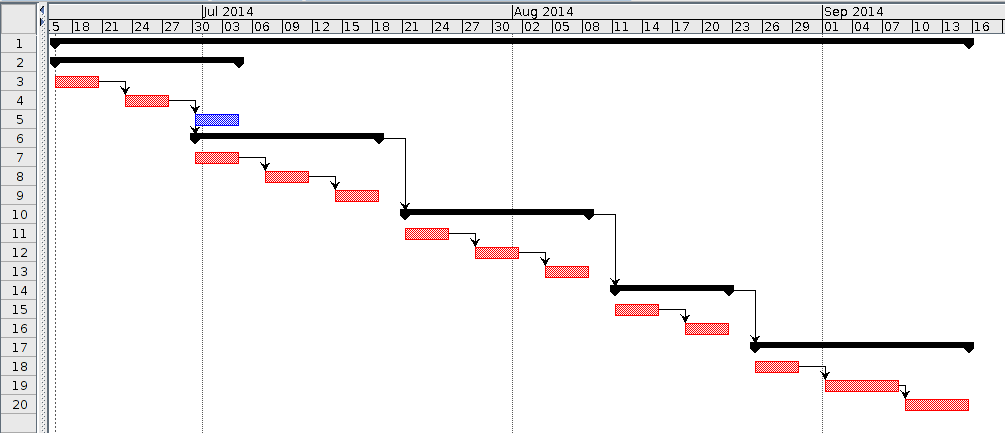
\includegraphics[width = 1\textwidth]{sample_project_gantt_1}
%     \caption{Sample project Gantt chart}
%   \end{figure}
% \end{frame}
% % Re-plan

\begin{frame}[t]\frametitle{Re-planning (if required!)}
\begin{itemize}
        \item Going back to your plan and making appropriate adjustments
        \item Should not be more than 10\% of your project's total effort
    \end{itemize}
\end{frame}
% section project_planning (end)

\section{Development methods} % (fold)
\label{sec:development_methods}
\begin{frame}[t]\frametitle{Development methods}
You have to pick one suitable methodology for your project and motivate it.
\begin{enumerate}
    \item Waterfall
     \item Agile
\end{enumerate}
\end{frame}
% section development_methods (end)

\section{Risk management} % (fold)
\label{sec:risk_management}
\begin{frame}[t]\frametitle{Risk management}
    \begin{itemize}
        \item Risk management is a important aspect of project management
        \item The goal risk management is to ensure that you are in a position to deal with these risk if they do occur and you are not facing them ill-prepared
        \item Major four stages of managing and controlling risks in your project are:
        \begin{description}
            \item[Identify risks]
            \item[Assess impact of risks]
            \item[Alleviate critical risks]
            \item[Control risks]
        \end{description}
    \end{itemize}
\end{frame}

\begin{frame}[t]\frametitle{1. Identify risks}
Risks can be of different types:
    \begin{itemize}
        \item Event-driven risks (hard disk crashing, etc.),
        \item Long term or chronic risks (bad estimation, etc.),
        \item Technical risks (unavailability of a particular library functions, etc.)
        \item Non-technical risks (illness, etc.)
    \end{itemize}
\end{frame}

\begin{frame}[t]\frametitle{2. Assess impact of risks}
    \begin{itemize}
        \item To estimate risks impact to your project, you can use following equation:
            $
            Impact = Likelihood * Consequence
            $
        \item Most serious risks are those which are highly likely to occur and have significant consequences

    %     \begin{figure}
    %       \centering
    %       \includegraphics[width = 0.9\textwidth]{likelihood}
    %       \caption{Likelihood and consequence scores }
        % \end{figure}
    \end{itemize}
\end{frame}

\begin{frame}[t]\frametitle{Risk likelihood and consequence scores~\cite{dawson2005projects}}
\begin{table}[htb!]
    \caption{Risk likelihood}
    \label{tab:risk_likelihood}
    \begin{center}
        \begin{tabular}{l|l}
        \hline

        \hline
        \textbf{Risk likelihood} & \textbf{Score}\\
        \hline
         Low   & 1 \\
         Medium & 2 \\
         High & 3 \\
        \hline

        \hline
        \end{tabular}
    \end{center}
\end{table}

\begin{table}[htb!]
    \caption{Risk consequence}
    \label{tab:risk_consequence}
    \begin{center}
        \begin{tabular}{l|l}
        \hline

        \hline
        \textbf{Risk consequence} & \textbf{Score} \\
        \hline
        Very low & 1 \\
        Low & 2 \\
        Medium & 3 \\
        High & 4 \\
        Very high & 5\\
        \hline

        \hline
        \end{tabular}
    \end{center}
\end{table}
\end{frame}

\begin{frame}[t]\frametitle{3. Alleviate critical risks}
 \begin{itemize}
        \item Three ways to deal with identified risks:
        \begin{description}
            \item [Avoidance] Reducing the chance of risk occurrence at all.
            \item [Deflection (transfer)] Passing the risk onto something or someone else.
            \item [Contingency] Accept that risk will occur and put something in place to deal with it when it does occur.
        \end{description}
    \end{itemize}
\end{frame}

\begin{frame}[t]\frametitle{4. Control risks}
    \begin{itemize}
        \item You can not just close your eyes now!
        \item Continuously monitor the risks as your project progresses and be prepared to deal with them.
    \end{itemize}
\end{frame}
% section risk_management (end)


\section{Configuration Management} % (fold)
\label{sec:configuration_management}

\begin{frame}[t]\frametitle{Configuration management}
    \begin{itemize}
        \item Common problems in software development projects are in the co-ordination and control associated with project artefacts.
        \item CM is used to preserve the old versions of the system
        \item To store artefacts efficiently
        \item A simple directory structure for configuration management is suggested!
        \item See the student's guide exercise 1!
    \end{itemize}
\end{frame}

% \begin{frame}[t]\frametitle{Sample project's configuration management approach}
% \begin{figure}[htb!]
%     \begin{center}
%         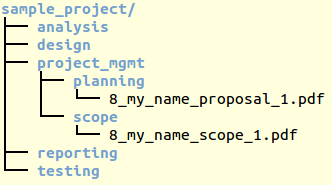
\includegraphics[width=4in]{cm_sample}
%     \end{center}
%     \caption{Sample project's configuration management approach}
%     \label{fig:cm_sample}
% \end{figure}
% \end{frame}
% section configuration_management (end)




% bibliography
\begin{frame}[t]\frametitle{References}
\cite{dawson2005projects}, \cite{weaver2004success}

\bibliography{../cp}
\bibliographystyle{plainnat}
\end{frame}

\end{document}
